L'attuale infrastruttura di rete si è stabilizzata per oltre un decennio e si è radicata profondamente nel contesto della società umana. Tuttavia, le imprese ed i fornitori di servizi stanno iniziando a realizzare i forti limiti e l'inflessibilità dello stato attuale dell'infrastrutura con le tecnologie di rete in rapida evoluzione e le crescenti richieste da parte degli utenti.

In altre parole si è riconosciuta la necessità di ristrutturare l'attuale architettura con qualcosa di più dinamico e flessibile \cite{suh2014building}.

\section{Software-Defined Network}\label{sdn}
Come risultato, per superare queste limitazioni intorno al 2005 è stata proposta la \textit{Software-Defined Network} (SDN). SDN è un concetto di rete che sta acquistando tendenza negli ultimi anni, il quale \textit{disaccoppia} il \textit{piano di controllo} e il \textit{piano dati}, \textit{centralizzando} così l'intelligenza di rete in un \textit{controller}.

L'idea di separare il controllo e il piano dati è nata principalmente con l'intenzione di permettere di sviluppare ciascuna parte in modo completamente indipendente l'una dall'altra, in modo che il software non sia vincolato dalla limitazione dell'hardware. Ed eventuali amministratori di rete possano orchestrare la rete per mezzo di applicazioni di alto livello, semplificandone la gestione \cite{fundation2012software}\cite{suh2014building}.

In altre parole si abbandona completamente la concezione verticale e monolitica di apparati di rete "tutto-in-uno", con l'intero stack (sia hardware e software) fornito da un'unica compagnia.
\newline
\newline
In caso di cambiamenti alla rete, anziché dover configurare manualmente ogni singolo switch in conformità di questi cambiamenti, è possibile utilizzare switch programmabili controllati da un'unica applicazione esterna.

\section{OpenFlow}\label{openflow}
Il componente più importante della SDN è un protocollo di comunicazione \textit{tra il piano di controllo ed il piano dati}. Il \textit{\textbf{protocollo OpenFlow}} è stato introdotto a tale scopo, supportato dalla \textit{Open Networking Foundation} (ONF); allo stato attuale, sono disponibili controller SDN open source che implementano OpenFlow, i più noti sono: \textit{NOX}, \textit{POX}, \textit{Ryu} e \textit{Floodlight} \cite{suh2014building}.

\section{Obiettivo}
Vista la nativa caratteristica delle SDN di effettuare azioni sul flusso del traffico, in particolare azioni come \textit{scartare} pacchetti (drop) o \textit{permetterne il passaggio} ed il diffuso utilizzo del protocollo OpenFlow, in questa relazione andremo a vedere alcune funzioni di firewall implementate tramite questa relativamente \textit{"nuova"} (2005!) architettura e protocollo ed ai possibili vantaggi e risvolte che è possibile avere sia nella sicurezza che nella gestione di reti.


\begin{figure}[H]
  \centering
    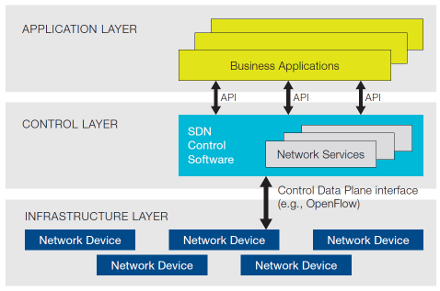
\includegraphics[width=\linewidth]{img/sdn-arch.png}
    \caption{Paradigma SDN}
  \label{fig:coffee}
\end{figure}
